
\noindent We have been on this journey from classical conformal symmetries to the implementation of the symmetries in a quantum setting. Thus far, we have found that the constraints of conformal symmetry in the context of quantum field theory, in $(2+0)$, $(1+1)$, and $(d+1)$ dimensions, the two-point correlation functions must decay polynomially as

\begin{equation}
\bra{0} \hat{\phi} (x) \hat{\phi} (y) \ket{0} \propto \frac{1}{|x-y|^\alpha}.
\end{equation}

\subsection*{Radial ``Quantization''}

\noindent Note that using quotes around quantization indicates that this approach is an inspired guess, and is not derived via a functor. \\

\noindent To build a quantum field theory with conforml symmetry, invariant under the group Conf$(\mathbb{R}^{2,0})$, we need four pieces of data. \\

\noindent (1) We need a Hilbert space $\mathcal{H}$ which is preferrably an infinite, separable, kinematic space of states isomorphic to the vector space of linear operators $L^2 (\mathbb{R})$, (2) a vacuum state, or a reference vector, $\ket{0}$, a subset of linear operators in the Hilbert space $\mathcal{L}(\mathcal{H})$ called \textit{observables} $\hat{\phi} (x,y)$, $(x,y) \in \mathbb{R}^2$, which are distribution-valued objects, but can be thought of, without harm, as self-adjoint operators. \\

\noindent The choice of set of observables, the subset of linear operators from the Hilbert space, define and distinguish a quantum field theory from others. E.g., the bosonic quantum field and the hydrogen atom share the same Hilbert space, but their observables are different and define what is allowed to be measured in each quantum field theory. \\

\noindent Our conformal quantum field theory yields (projective) unitary representations of Conf$(\mathbb{R}^{2,0})$. We can use analytic continuation to map to a Minkowski theory where we have representations of Conf$(\mathbb{R}^{1,1})$. \\

\noindent Introduce the construction of ``imaginary time''

\begin{equation}
\begin{pmatrix} x \\ y \end{pmatrix} \rightarrow \begin{pmatrix} x \\ it \end{pmatrix}; \,\, t \in \mathbb{R}.
\end{equation}

\noindent If possible, the correlation functions analytically continue, such that

\begin{equation}
\bra{0} \hat{\phi} (x,y) \hat{\phi} (0,0) \ket{0} = f(x,y) \rightarrow f(x,it).
\end{equation}

\noindent If all $n$-point correlation functions are analytically continued in this way, it \textit{often} happens that we get a mapping

\begin{equation}
G^{(n)} ((x_1,y_1), \dots) \rightarrow G^{(n)} ((x_1,t_1), \dots)
\end{equation}

\noindent Which are invariant, respectively, under symmetry transformations

\begin{equation}
\text{Conf}(\mathbb{R}^{2,0}) \rightarrow \text{Conf}(\mathbb{R}^{1,1}).
\end{equation}

\noindent This is the analytic continuation to a \textit{Minkowski theory}, and the criteria to ensure that this mapping exists is called \textit{reflection positivity}. See the work of Glimm and Jaffe for a rigorous account of this machinery. \\

\noindent With a Minkowski quantum field theory, enter the Heisenberg picture to apply time evolution, and analytically continue the ``time'' variable to define ``inverse temperature'' $t \rightarrow -i\beta$, which essentially gives the correlation function for the thermal state of the Hamiltonian $\hat{H}$ with inverse temperature $\beta$

\begin{align}
\bra{0} \hat{\phi} (x,y) \hat{\phi} (0,0) \ket{0} &= \bra{0} e^{-it \hat{H}} \hat{\phi} (x,0) e^{it\hat{H}} \hat{\phi} (0,0) \ket{0} \\
&= \bra{0} e^{-\beta \hat{H}} \hat{\phi} (x,0) e^{\beta \hat{H}} \hat{\phi} (0,0) \ket{0}.
\end{align}

\noindent \textbf{Digression}: What does ``physical'' mean for this course? \\

\noindent To define a physical theory, we require \textit{kinematics} and \textit{observables}, which make for a perfectly fine physical theory, even without \textit{dynamics}. \\

\noindent The kinematics of a system introduces a Hilbert space $\mathcal{H}$ and a set of density operators $\rho(\mathcal{H})$ that describe the states of the system, but do not allow measurement of those states. The observables of a system $\mathcal{O} \subset \mathcal{L}(\mathcal{H})$ are the measurements of the states of the system, and are labelled by points in the underlying manifold $\mathcal{M}$ of the theory, such that $x, x^\dagger, \mathbb{I} \in \mathcal{O}, \, \text{ for } x \in \mathcal{M}$. \\

\noindent Dynamics of a system are introduced via the group of isometries on the manifold $G = \text{Isom}(\mathcal{M})$, and, for a quantum field theory, we search for projective, unitary representations of $G$ on the Hilbert space. The construct of time only comes in as a choice of the manifold and its one-dimensional subgroups that act like time, but time is not necessarily an axiom of a quantum theory. \\

\noindent \textbf{End Digression}. \\

\noindent So far, we have labelled our observables in our Minkowski CFT by $(\sigma^0, \sigma^1) \in \mathbb{R}^{1,1}$. We now complexify these coordinates by ``Euclideanizing'' and sending the timelike coordinate to be imaginary, such that $\sigma^0 \rightarrow i \sigma^0$, and 

\begin{equation}
z = \sigma^1 + i \sigma^0 \text{ and } \bar{z} = \sigma^1 - i \sigma^0
\end{equation}

\noindent Which correspsonds to an analytic continuation of the $n$-point correlation functions

\begin{equation}
G^{(n)} (\underline{\sigma}_1, \underline{\sigma}_2, \dots) \rightarrow G^{(n)} (\underline{z}_1, \bar{\underline{z}}_1; \underline{z}_2, \bar{\underline{z}}_2; \dots).
\end{equation}

\noindent In this complexifed, Euclidean spacetime, with locations defined by coordinates $z$ and $\bar{z}$, compactify space to a cylinder, such that space corresponds to the transverse direction $\sigma^1 \rightarrow \sigma^1 + 2\pi$, and time corresponds to the longitudinal direction, and our complex coordinates are now

\begin{equation}
z = e^{\sigma^1 + i \sigma^0} \text{ and } \bar{z} = e^{\sigma^1 - i \sigma^0}.
\end{equation}

\noindent Circles in the complex plane correspond to constant time, the radial direction on the cylinder, and the real coordinates $\sigma^0, \sigma^1$ are mapped to the complex coordinates as

\begin{equation}
\sigma^0 = \infty \rightarrow z = \infty \text{ and  } \sigma^0 = -\infty \rightarrow z=0
\end{equation}

\noindent And transformations maps as

\begin{align}
\text{Time reversal } [\sigma^0 \rightarrow -\sigma^0] &\rightarrow \text{Inversion } [z \rightarrow \frac{1}{z}] \\
\text{Time translation } [\sigma^0 \rightarrow \sigma^0 + a] &\rightarrow \text{Dilation } [z \rightarrow e^a z] \\
\text{Spatial translation } [\sigma^1 \rightarrow \sigma^1 + a] &\rightarrow \text{Rotation } [z \rightarrow e^{ia} z] 
\end{align}

\begin{figure}[H]
	\centering
	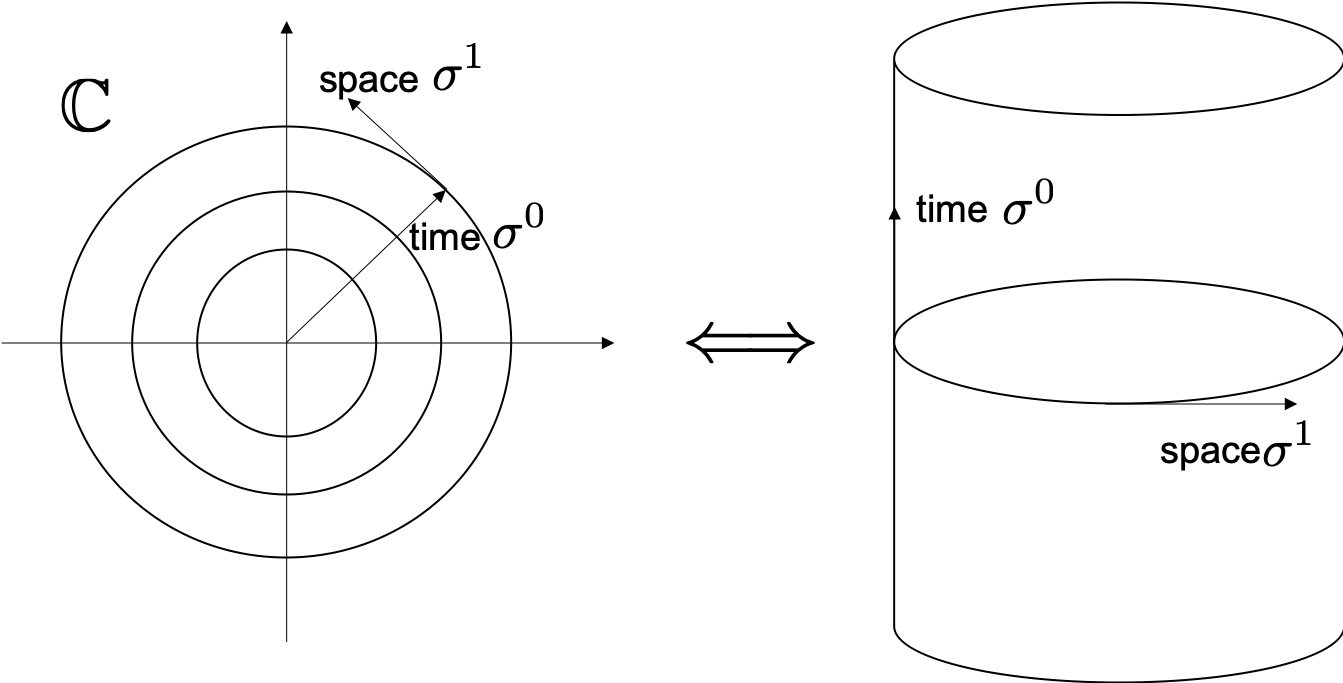
\includegraphics[width=3.5in]{images/radial_quantization.png} 
\end{figure} 

\noindent Now we make a move to constructing a conformal field theory in complexified, Euclidean spacetime. \\

\subsection*{Ward Identities}

\noindent Witha conformally invariant classical theory, we work towards getting a collection of observables obeying the correct symmetry for a conformally invariant quantum theory. \\

\noindent Recall from Noether's theorem that conserved charges correspond to classical symmetries $Q$ obeying the anticommutation bracket

\begin{equation}
\{ Q_j, Q_k \} = f_{jk}^{\,\,\,\,l} Q_l.
\end{equation}

\noindent We may try to naively quantize by ``puttings hats on'' the conserved quantities that obey the commutation brackets

\begin{equation}
[ \hat{Q}_j, \hat{Q}_k ] = i f_{jk}^{\,\,\,\,l} \hat{Q}_l,
\end{equation}

\noindent But without a Hilbert space, we can not write these operators as functions of the fields (e.g., $\hat{Q} = f(\hat{\phi})$. \\

\noindent From the classical symmetries, we now derive the quantum generators of the symmetries. \\

\noindent Suppose we have a classical field theory with action $S[\underline{\phi}]$, where $\underline{\phi}$ is a vector of classical fields. Assume that $S$ is symmetric under the Lie group of infinitesimal transformations, such that

\begin{equation}
\underline{\phi}' (\underline{x}) = \underline{\phi} (\underline{x}) - i \omega_a (\underline{x}) \textbf{G}_a \underline{\phi} (\underline{x}) = e^{-i \omega_a (\underline{x}) \textbf{G}_a} \underline{\phi} (\underline{x})
\end{equation}

\noindent Where $\omega_a (\underline{x})$ is infinitesimal and $\textbf{G}_a$ is a matrix acting on the vector labels of $\underline{\phi}$. \\

\noindent Use the path integral prescription to work out how this transformation affects the correlation functions

\begin{equation}
\bra{0} \underline{\hat{\phi}} (\underline{x}_1) \dots \underline{\hat{\phi}} (\underline{x}_n) \ket{0} = \lim_{T \rightarrow \infty(1-i\epsilon)} \frac{\int \mathcal{D}\phi \, \phi (\underline{x}_1) \dots \phi (\underline{x}_n) e^{iS[\underline{\phi}]}}{\int \mathcal{D} \phi \, e^{i S[\underline{\phi}]}}.
\end{equation}

\noindent The first step is to change variables $\underline{\phi} \rightarrow \underline{\phi}'$ and assume that the measure is invariant $\mathcal{D}\phi' = \mathcal{D}\phi$. Define the operator $\hat{X}$ to be the time-ordered product of quantum fields

\begin{equation}
\hat{X} = \mathcal{T} [ \underline{\hat{\phi}} (\underline{x}_1) \dots \underline{\hat{\phi}} (\underline{x}_n)].
\end{equation}

\noindent Note that the time-ordering will be assumed from here on, and consider the expectation value of $\hat{X}$ in the path integral prescription

\begin{equation}
\langle \hat{X} \rangle = \frac{\int \mathcal{D} \phi' \, \left( \underline{\hat{\phi}} (\underline{x}_1) \dots \underline{\hat{\phi}} (\underline{x}_n) + i \omega_a (\underline{x}) \textbf{G}_a (\underline{\hat{\phi}} (\underline{x}_1) \dots \underline{\hat{\phi}} (\underline{x}_n) + \dots \right) e^{i (S + \int dx \, \partial_\mu j_a^\mu \omega_a (\underline{x}))}}{\int \mathcal{D}\phi \, e^{iS}}.
\end{equation}

\noindent To zeroth order in $\omega_a$, this is exactly the correlation function prior to the change of variables. To first order in $\omega_a$, we get the equality for quantum fields

\begin{equation}
\frac{\partial}{\partial x^\mu} \langle \hat{j}_a^\mu (\underline{x}) \hat{\phi} (\underline{x}_1) \dots \hat{\phi} (\underline{x}_n) \rangle = -i \sum_{j=1}^{n} \delta(\underline{x} - \underline{x}_j) \langle \hat{\phi} (\underline{x}_1) \dots \textbf{G}_a \hat{\phi} \left( \underline{x}_j) \dots \hat{\phi} (\underline{x}_n) \right)\rangle.
\end{equation}

\noindent The generator of symmetry $\hat{j}_a^\mu (\underline{x})$ is handed over by the oath integral approach.